\documentclass[../main.tex]{subfiles}
\begin{document}

Bei der Entwicklung von dem Feature wurde viel lokal getestet, da Tests in \glspl{glos:pipeline} viel Zeit kosten.
So war eine Herausforderungen, dass sich die geschriebenen Code Scripte anders in den beiden Umgebungen verhalten.

\begin{figure}[ht]
    \centering
    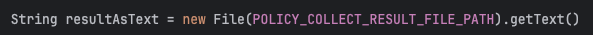
\includegraphics[scale=0.45]{bilder/codebad.png}
    \caption{Beispiel Script für Code, der nicht in einer \gls{glos:pipeline} funktioniert}
    \footnotesize (selbst geschrieben)
    \label{fig:codebad}
\end{figure}


In dem Beispiel Script in Abbildung \ref{fig:codebad} ist zu sehen, wie mit einer standard Java Funktionalität die Auswertungsergebnisdatei gelesen wird.
Dieses Implementierung funktioniert lokal problemlos, scheitert aber in einer \gls{glos:pipeline}, da diese Java Funktionalität nicht in der \gls{glos:pipeline} Umgebung verfügbar ist.

\begin{figure}[ht]
    \centering
    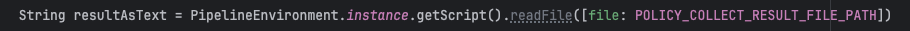
\includegraphics[scale=0.45]{bilder/codegood.png}
    \caption{Beispiel Script für Code, der \gls{glos:pipeline} Funktionalität benutzt}
    \footnotesize (selbst geschrieben)
    \label{fig:codegood}
\end{figure}
        
Um dieses Problem zu umgehen, stehen dafür Funktionalitäten von der \gls{glos:pipeline} Umgebung zu Verfügung.
Der Aufruf aus Abbildung \ref{fig:codegood} zeigt wie so eine Funktionalität benutzt werden kann.
Bei dieser Implementierung ist zu beachten, dass sie vorerst nur in der \gls{glos:pipeline} funktioniert.
Lokal besteht die Möglichkeit bei diesem Aufruf im Hintergrund den Code aus Abbildung \ref{fig:codebad} auszuführen, damit auch weiterhin getestet werden kann.
Alle Code Abschnitte, die mit Dateien arbeiten, mussten entsprechend angepasst werden.

Durch diese Herausforderung ist das Verständnis für die Funktionsweise von \glspl{glos:pipeline} und das Bewusstsein für die Bedeutung der Umgebung, in der gearbeitet wird, gewachsen.
\end{document}

